
\begin{frame}
    \frametitle{Testdatensatz}
    \begin{center}
    \huge{Probleme}
    \end{center}
\end{frame}

\begin{frame}
  \frametitle{Falsche Datensätze}
  \Wider{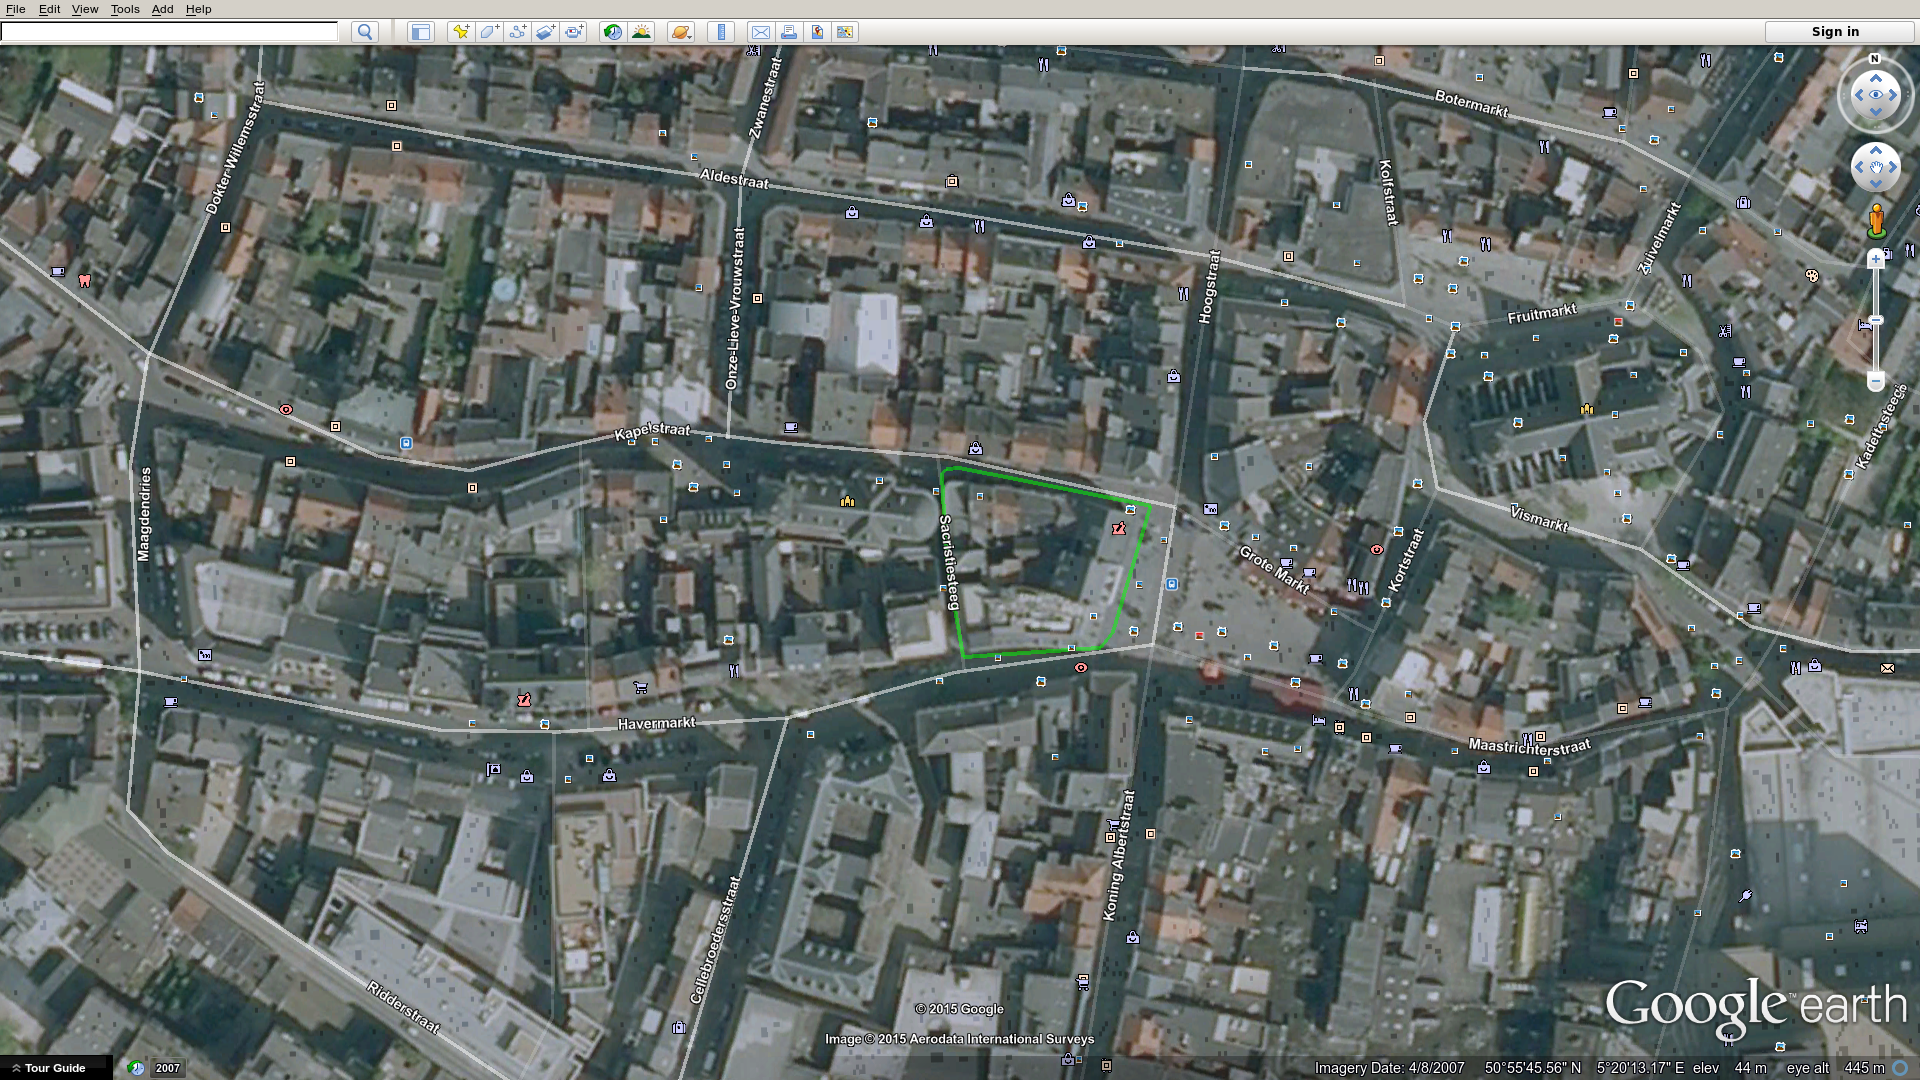
\includegraphics[width=\textwidth]{40_fail_earth}}
\end{frame}

\begin{frame}
  \frametitle{Falsche Datensätze}
  \Wider{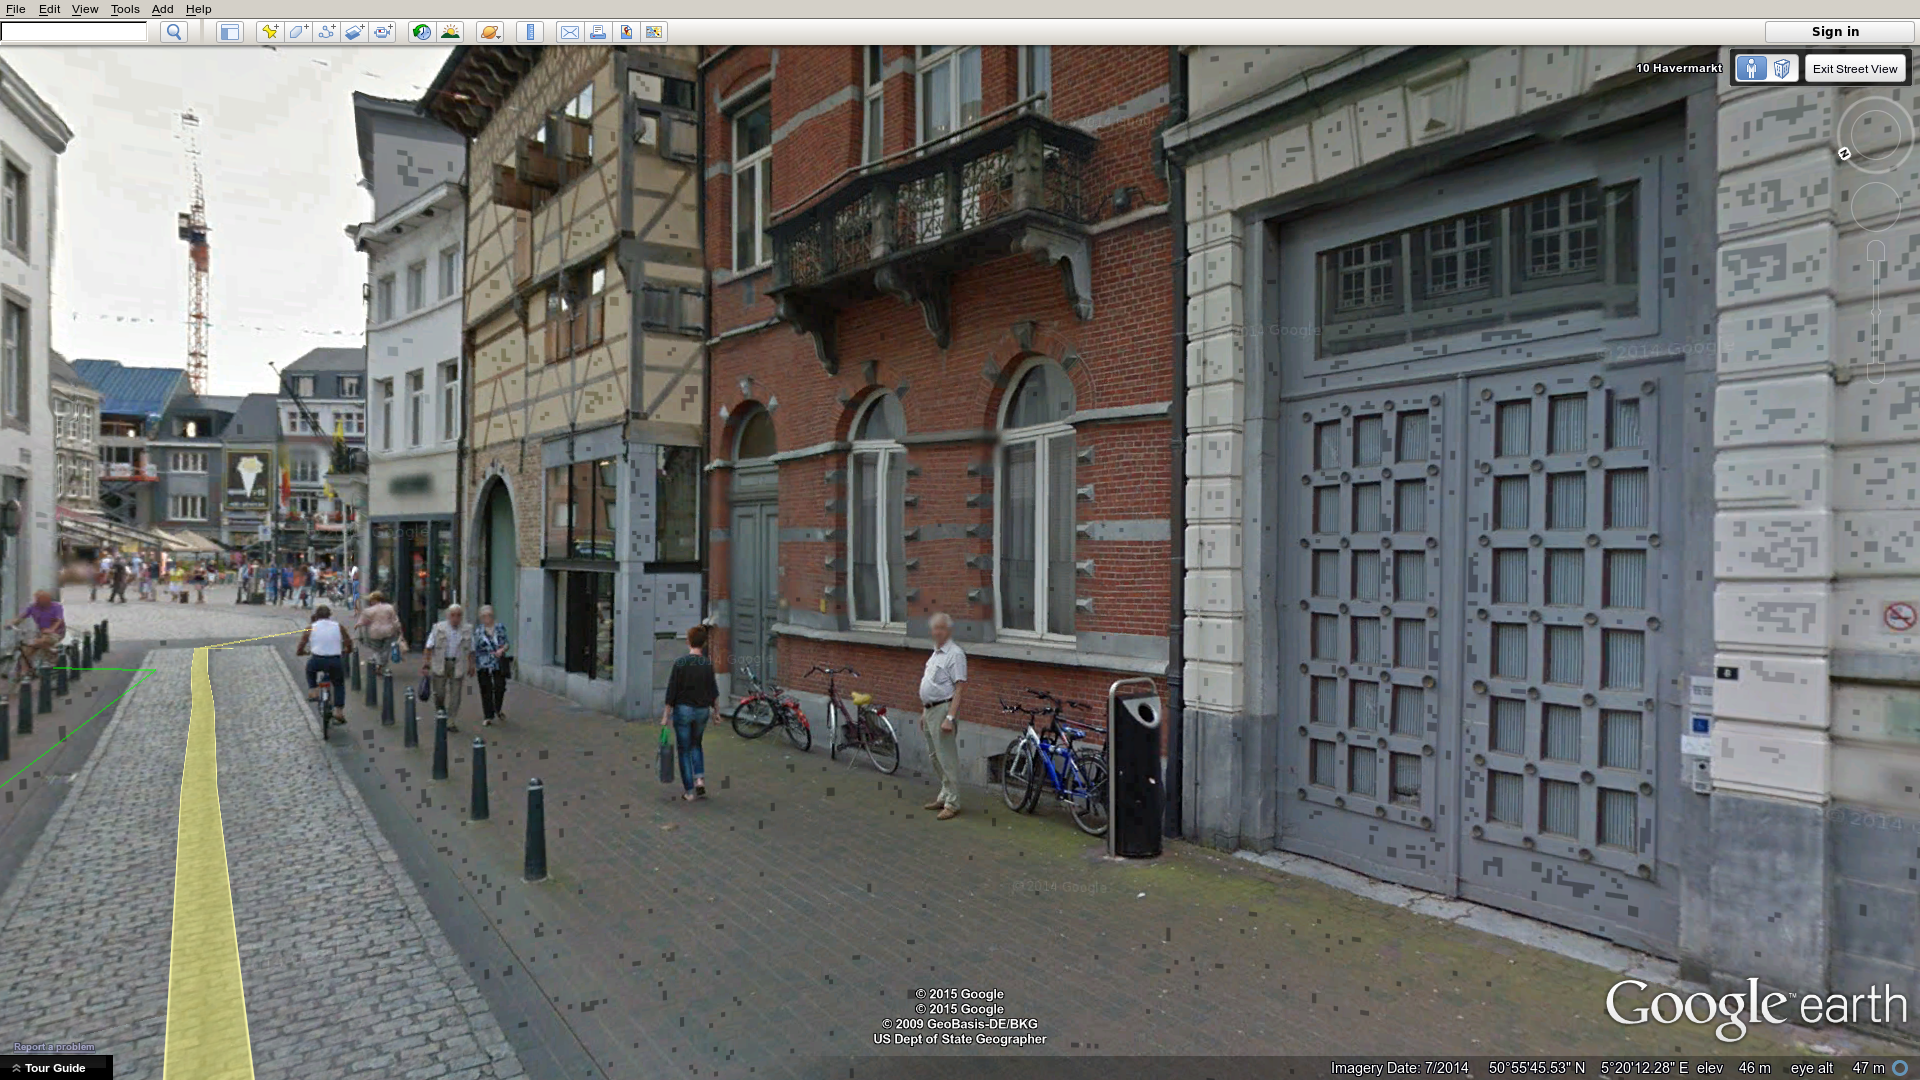
\includegraphics[width=\textwidth]{40_fail_street}}
\end{frame}

\begin{frame}
  \frametitle{Falsche Datensätze}
  \Wider{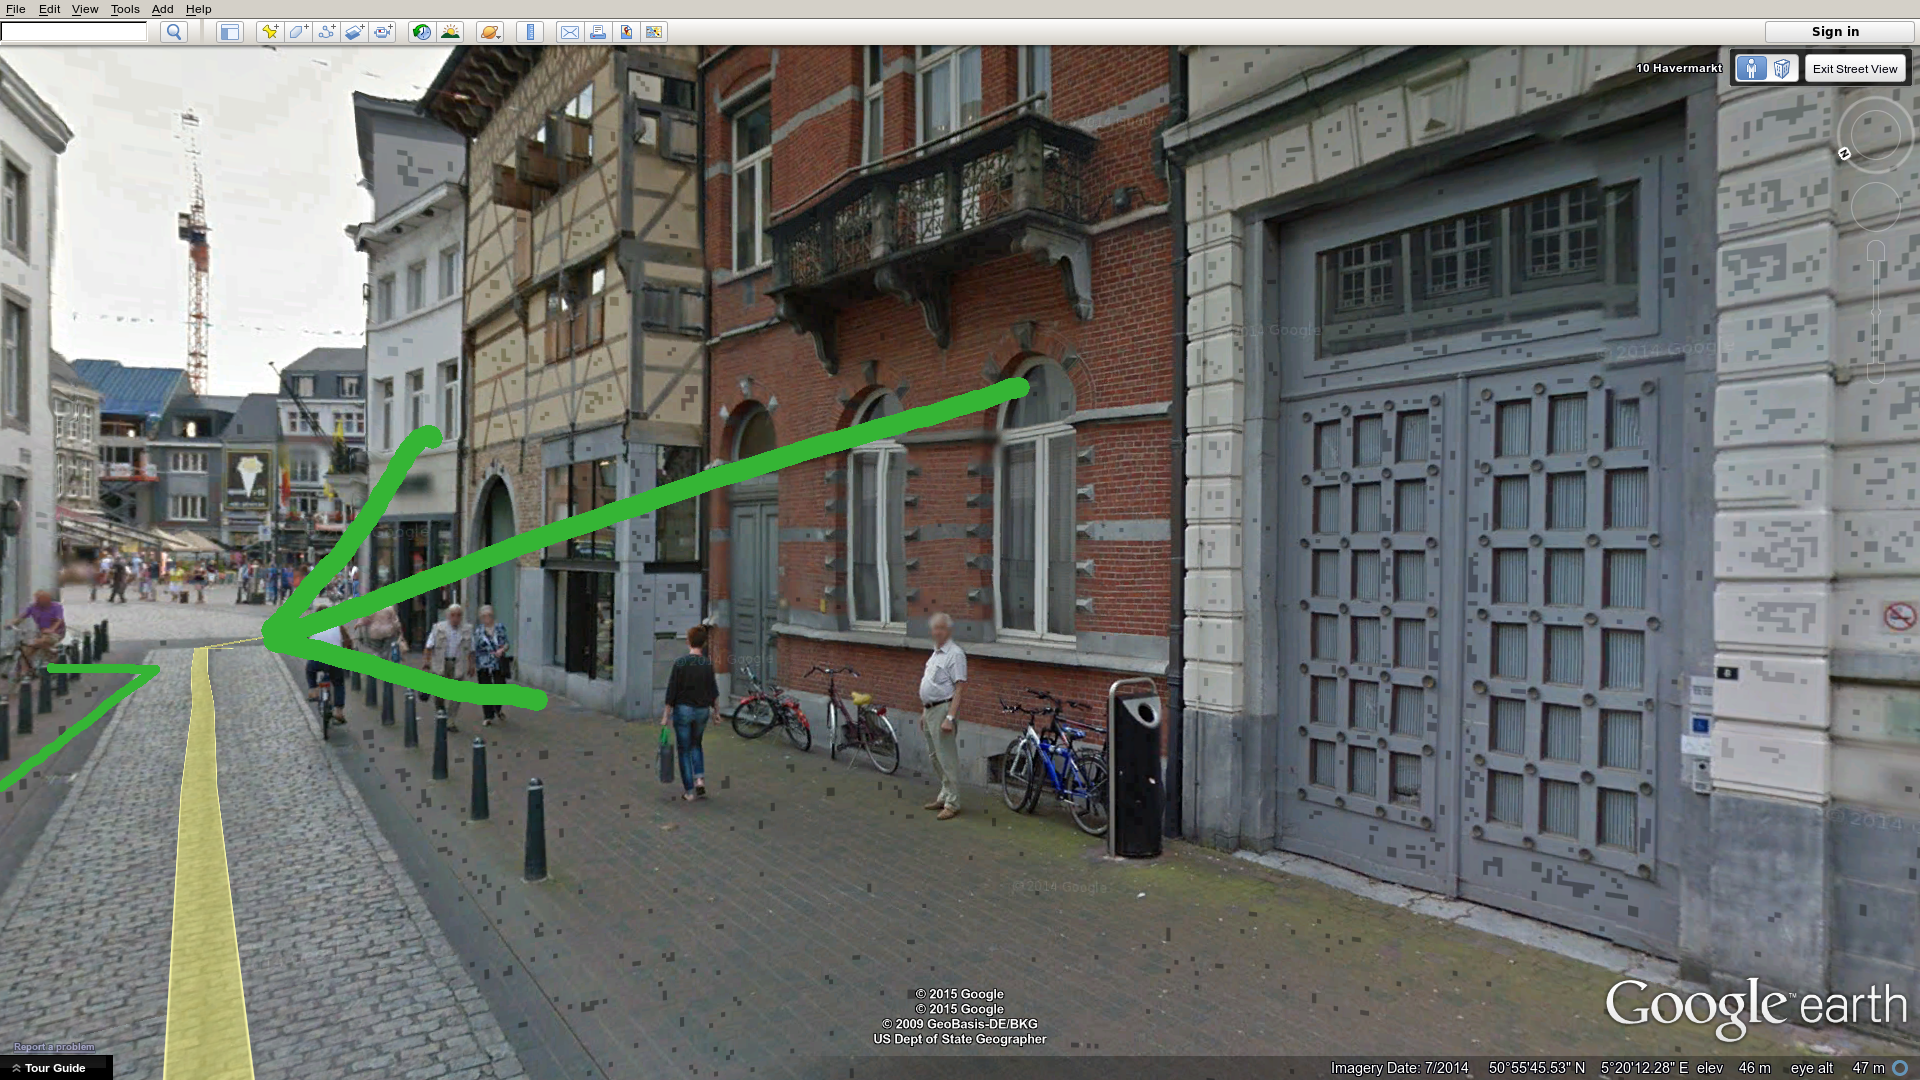
\includegraphics[width=\textwidth]{40_fail_street_building}}
\end{frame}

\begin{frame}
  \frametitle{Falsche Datensätze}
  \Wider{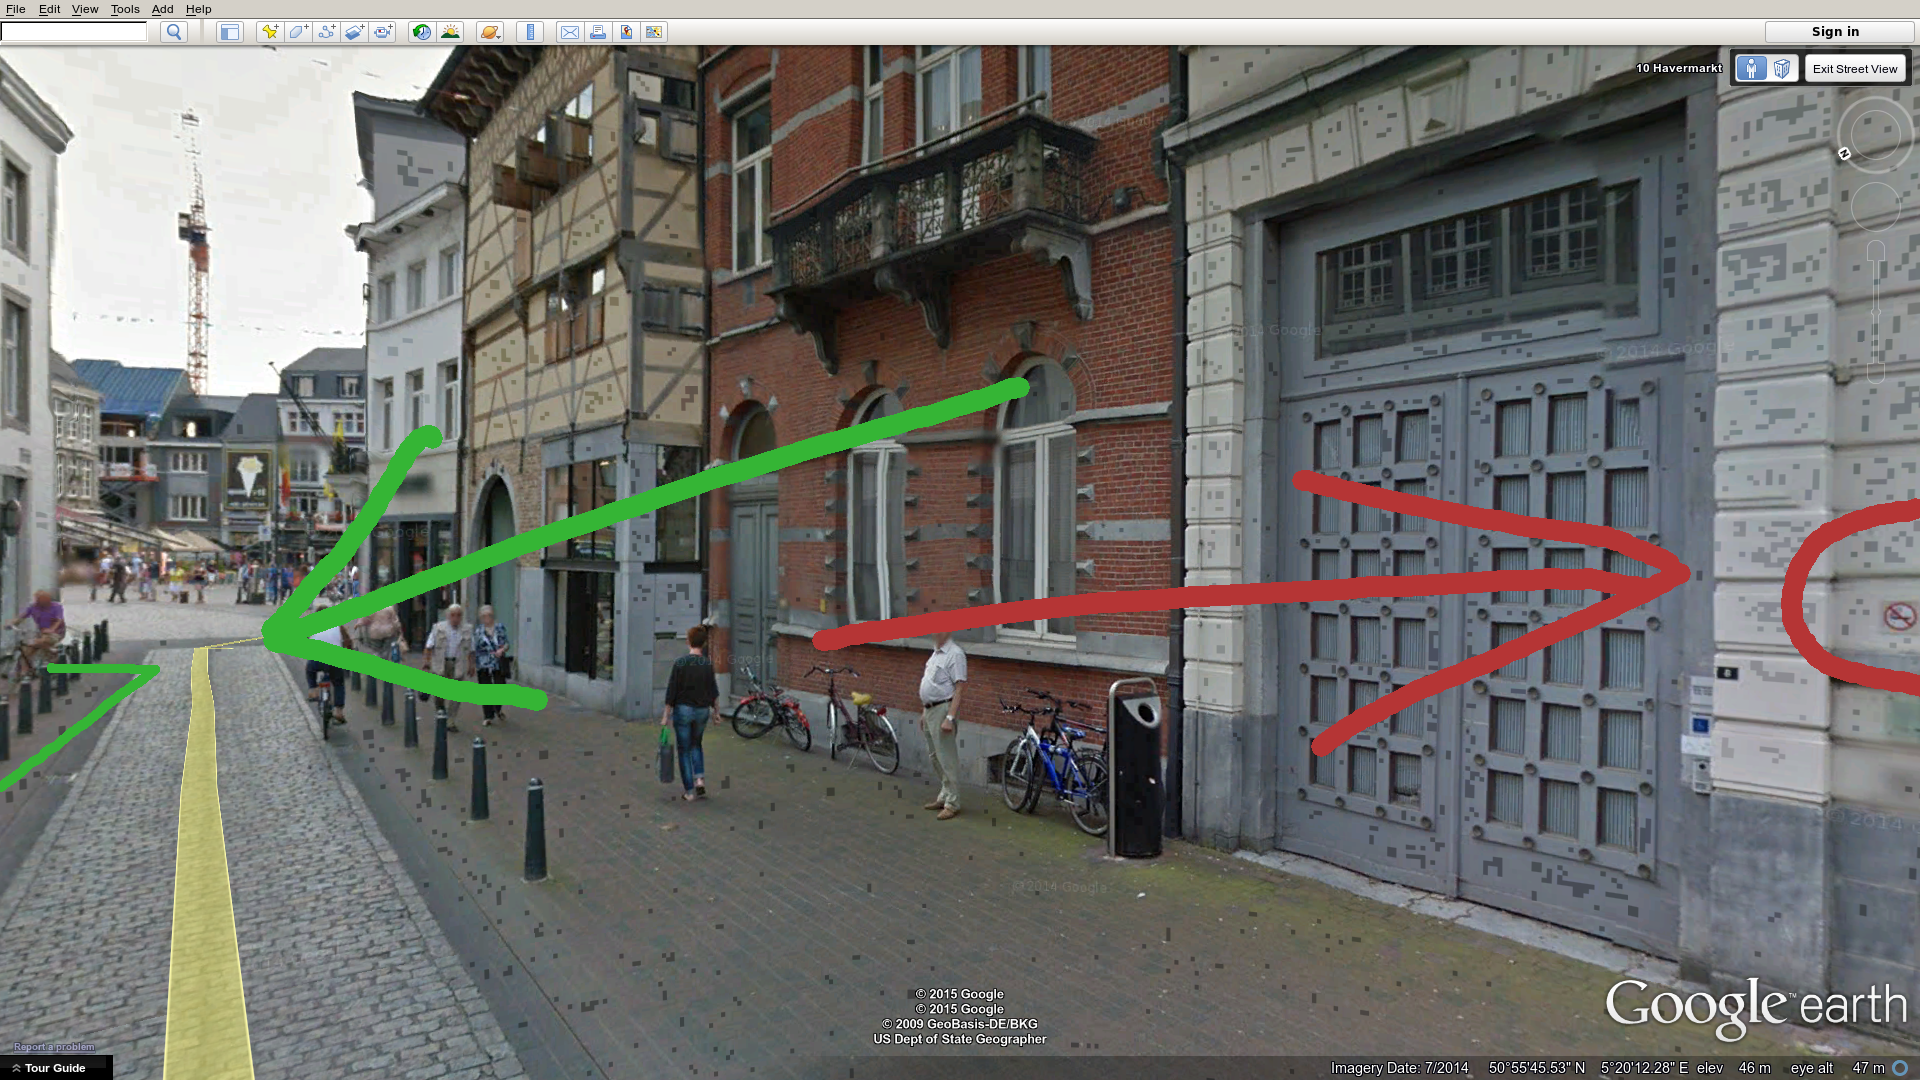
\includegraphics[width=\textwidth]{40_fail_street_sign}}
\end{frame}

\begin{frame}
  \frametitle{Falsche Datensätze}
  \Wider{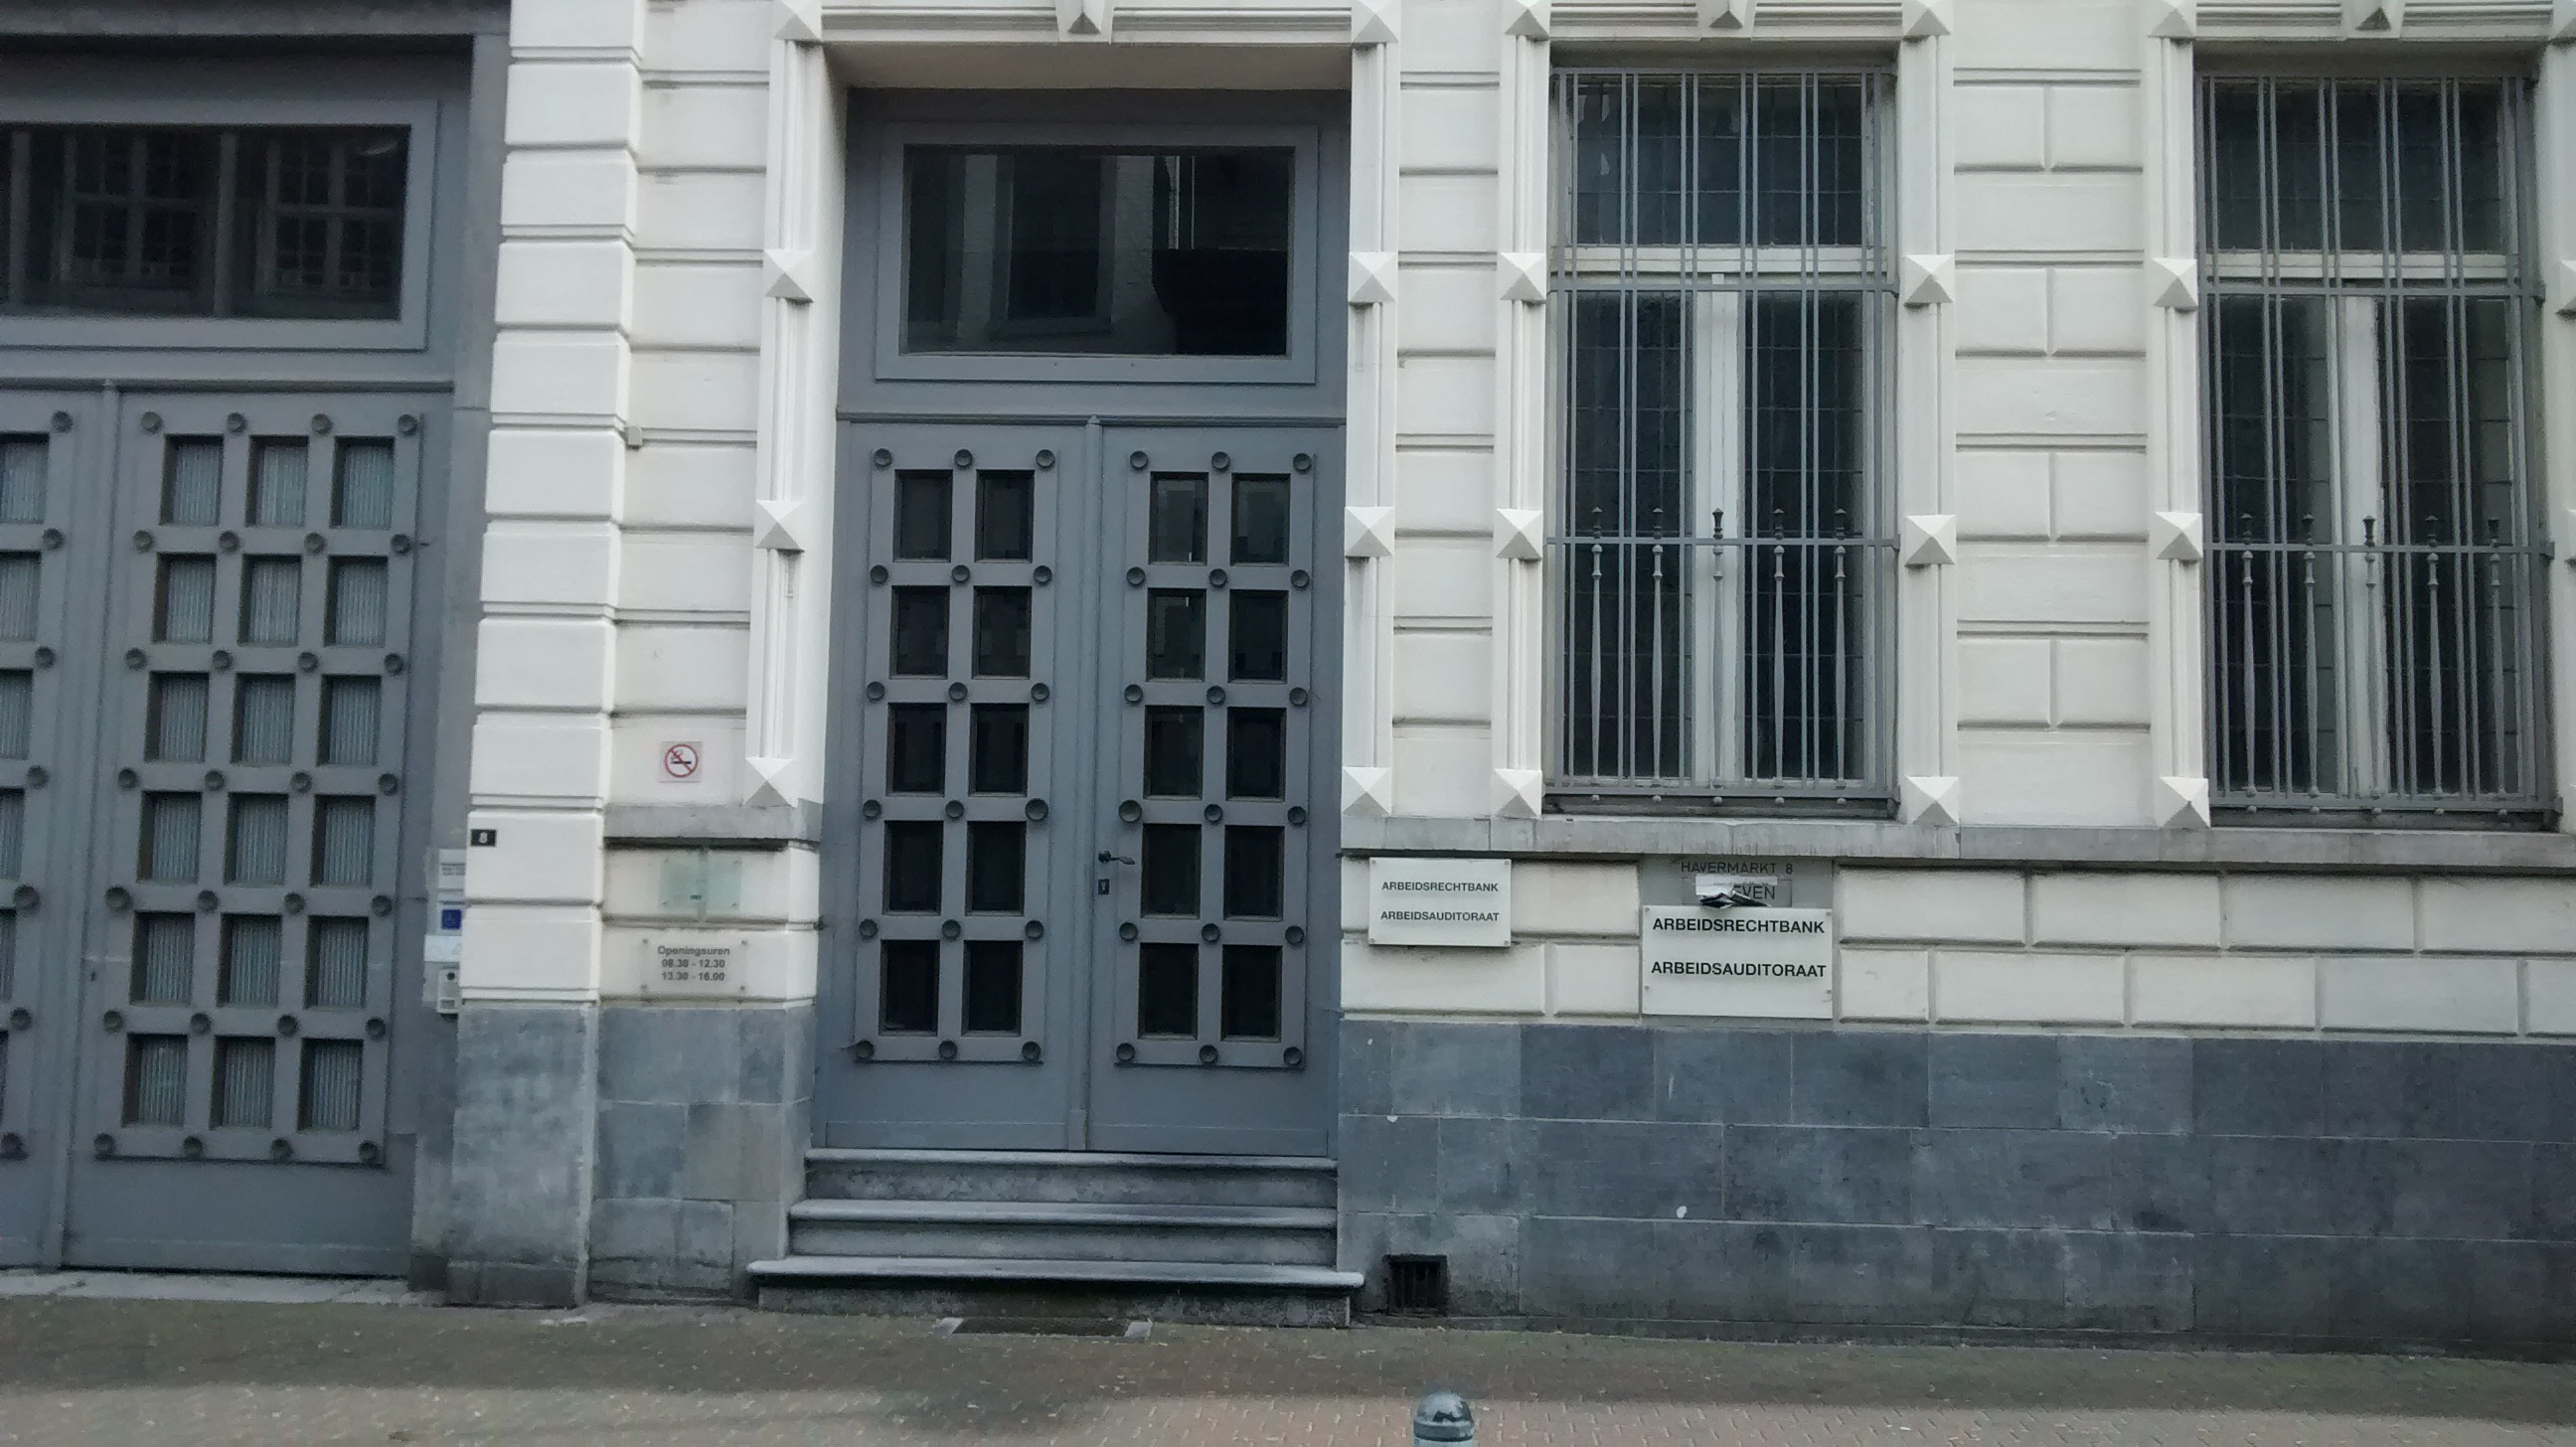
\includegraphics[width=\textwidth]{0040}}
\end{frame}


\begin{frame}
  \frametitle{Unvollständige Datensätze}
  \Wider{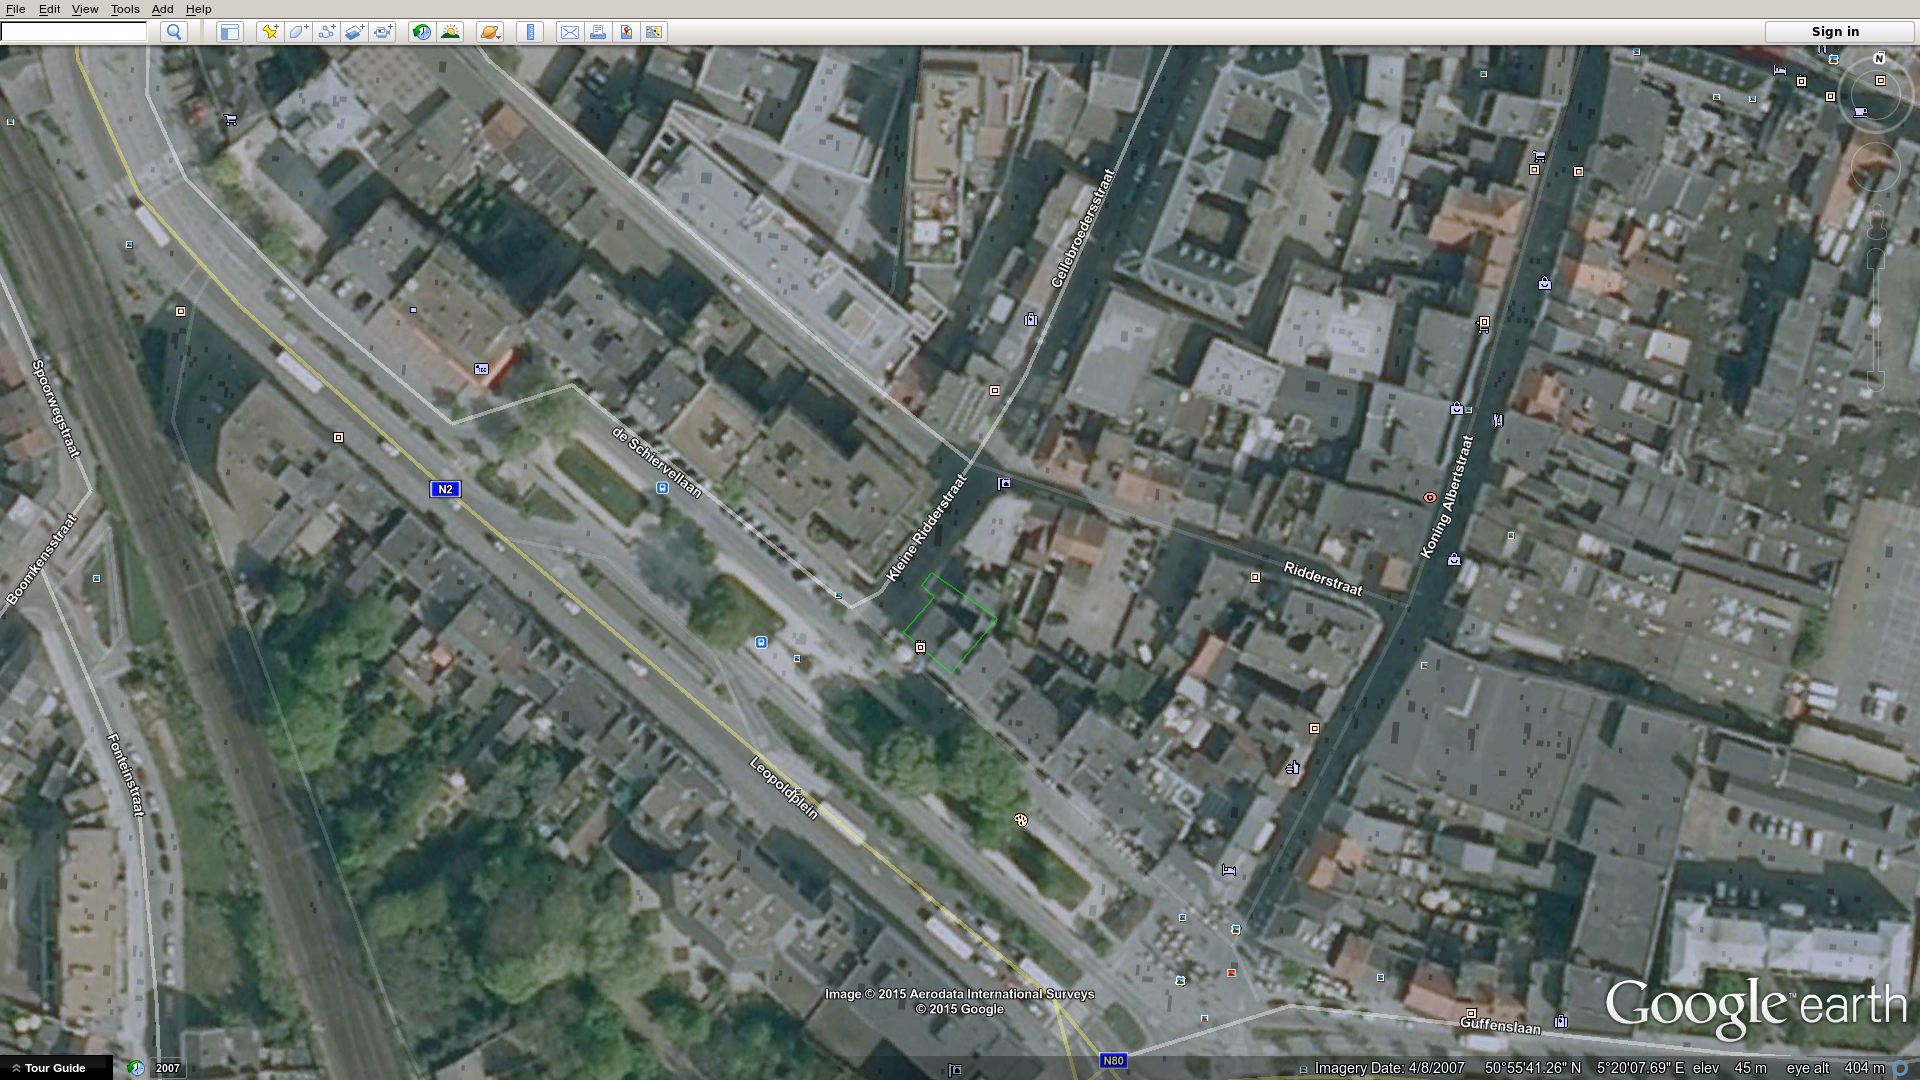
\includegraphics[width=\textwidth]{google_earth}}
\end{frame}

\begin{frame}
  \frametitle{Unvollständige Datensätze}
  \Wider{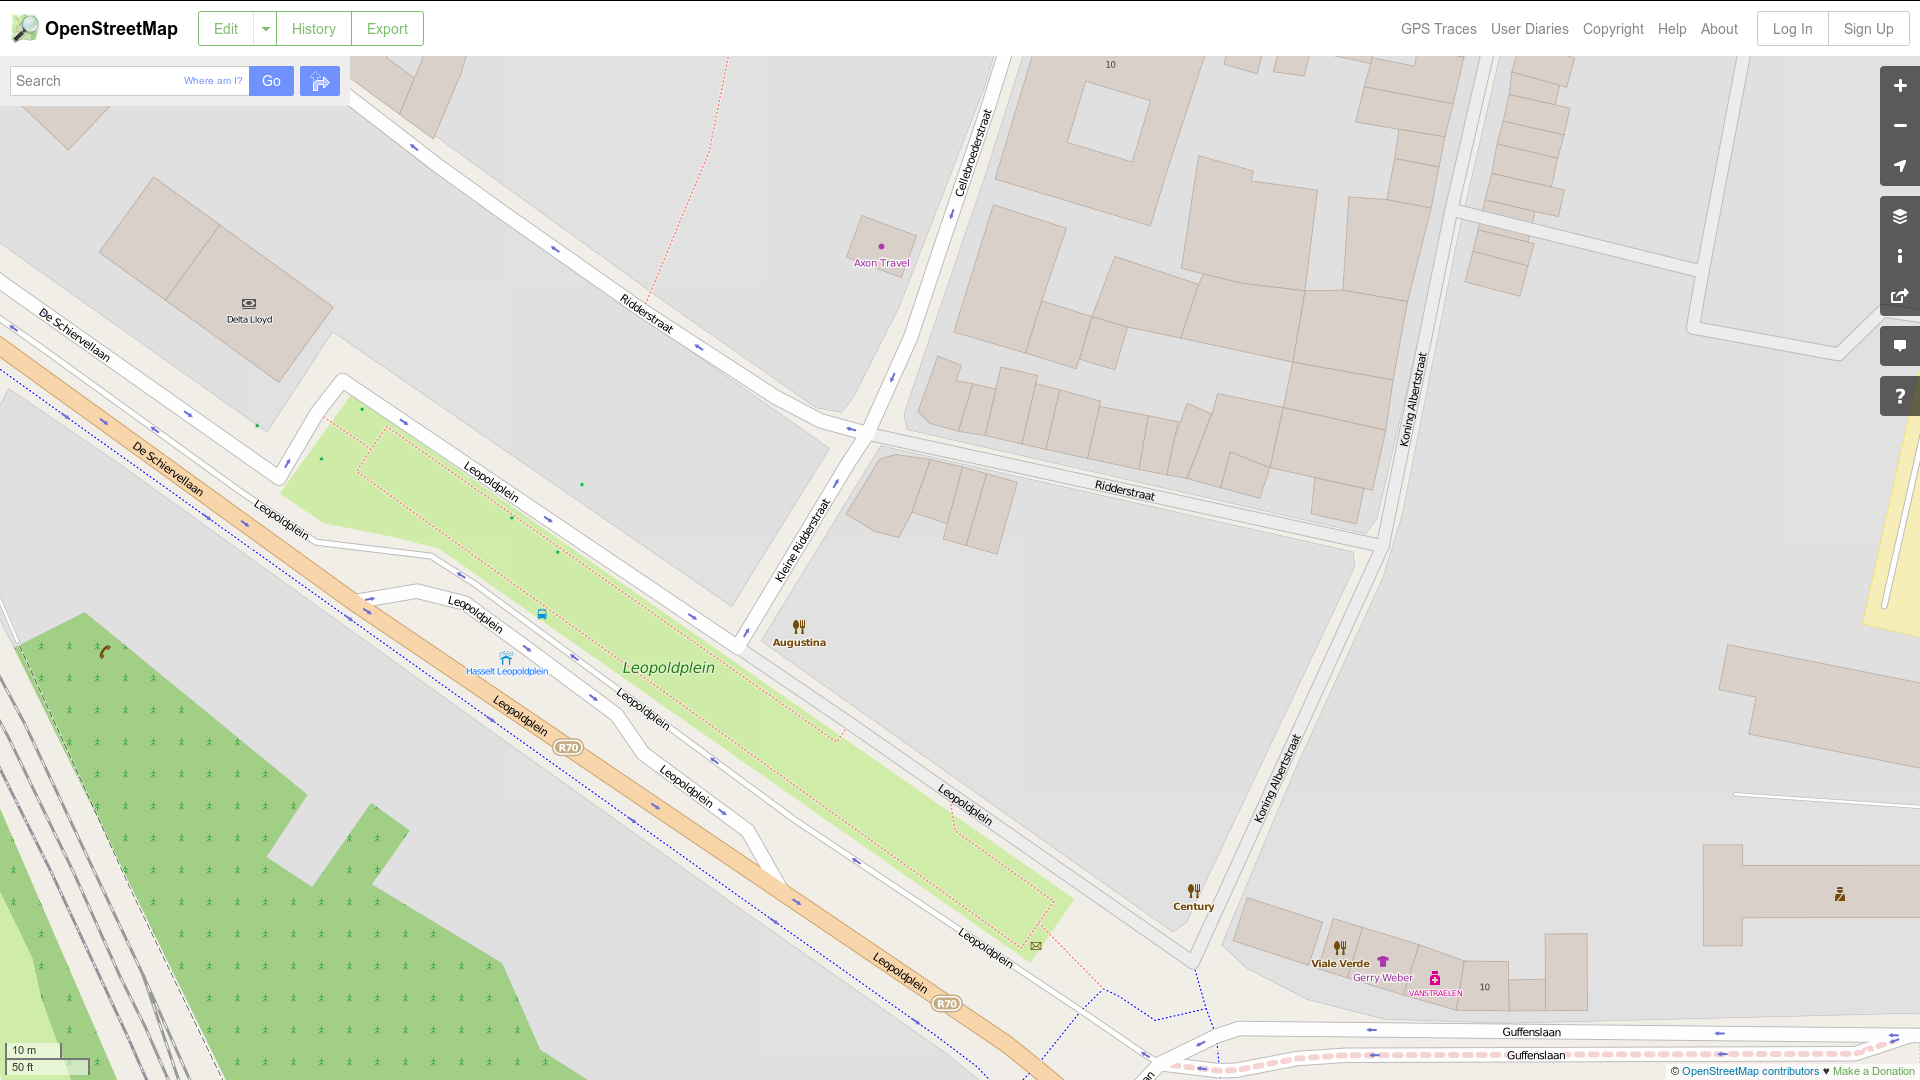
\includegraphics[width=\textwidth]{unvollstaendig}}
\end{frame}



\begin{frame}
    \frametitle{Datensatz untersuchen}
    % Bild von OpenStreetMap von unvollständigen Daten
    % weitere Beispiele von falschen Daten
\end{frame}

\begin{frame}
    \frametitle{Fehlerbereinigung}
    %
    %Content goes here
\end{frame}

\begin{frame}
    \frametitle{Idee zur Android-App}
    %Content goes here
\end{frame}

\begin{frame}
    \frametitle{Darstellung des Datensatzes}
    %Content goes here
\end{frame}
